\documentclass[twocolumn]{aastex631}
\usepackage{subfigure}
\graphicspath{{./pictures/}}

\begin{document} 

   \title{Constraint result to the self-interacting dark matter model without dark energy
   in cosmology}

   \author{Yixuan Zhu}\affiliation{Department of Astronomy, Beijing Normal University.
   Beijing 100875.
   PR China}
 
   \begin{abstract}

   \end{abstract}
   
   \keywords{}

\section{Introduction}

   The standard Λ-Cold Dark Matter (ΛCDM) model has been successful in 
   explaining the accelerated expansion of the Universe (\cite{Riess_1998,Perlmutter_1999}), 
   from the cosmic microwave background (CMB) anisotropies (\cite{Bennett_1996}) to 
   the measurement of baryon acoustic oscillations (BAO; \cite{Eisenstein_2005}). 
   However, there are also many alternative models that have been proposed to describe 
   the phenomenon, such as the canonical ``quintessence" scalar field theories 
   (\cite{PhysRevD.37.3406, WETTERICH1988668,PhysRevLett.80.1582}),
   non-canonical ``k-essence" theories (\cite{PhysRevLett.85.4438, PhysRevD.63.103510})
   and the modified gravity models (see, e.g., \cite{CLIFTON20121} for a review).

   It has been shown that dark matter self-interaction could contribute 
   to the accelerated expansion without dark energy component (\cite{PhysRevD.64.063501, Balakin_2003}). 
   According to the Boltzmann formalism, the disequilibrium between dark matter particle
   creation and annihilation processes would creat an effective source term 
   making negative pressure just like the dark energy. \cite{Basilakos_2009}
   investigated the analytical solutions for the simple interacting dark matter (IDM) 
   model, and find that the effective annihilation term is much smaller than the
   results given by the general methods. The gravitational matter creation model (\cite{Lima_2008})
   is mathematically equivalent to one case of the IDM models (\cite{Basilakos_2009}).

   In this paper, we use the newly revised data from $H(z)$, supernovae Ia, 
   quasars and baryon acoustic oscillation by using the Markov chain Monte
   Carlo (MCMC) method. The result gives that the lower limit of the interacting
   dark matter particle mass is about 1 eV.

\section{The basic equations in the IDM model}

   We assume that the total density of the cosmic fluid obeys
   the collisional Boltzmann equation (\cite{Kolb:1990vq})
   \begin{equation}
      \dot{\rho}+3H\rho+\kappa\rho^2-2\Psi=0,
   \end{equation}
   where $\rho$ is the total energy-density of the cosmic fluid,
   containing dark matter, baryons, and any type of exotic energy,
   $\Psi$ is the rate of creation of DM particle pairs, and the
   annihilation parameter $\kappa(\geq0)$ is given by:
   \begin{equation}
      \kappa=\frac{\langle\sigma u\rangle}{M_x},\label{eq:2}
   \end{equation}
   where $\sigma$ is the cross-section for annihilation, $u$ is
   the mean particle velocity, and $M_x$ is the mass of the DM
   particle.
   Compared to the usual fluid equation, the effective pressure term
   is \begin{equation}
      P=\frac{\kappa\rho^2-\Psi}{3H}.
   \end{equation}
   When $\kappa\rho^2-\Psi<0,$ what means that the IDM particle
   creation term is larger than the annihilation item, IDM may serve
   as a negative pressure source in the global dynamics of the Universe,
   like the role of Dark Energy in the general cosmological models.

   \cite{Basilakos_2009} identified two functional forms for which
   the previous Boltzmann equation can be solved analytically.
   Refering to Appendix B in \cite{Basilakos_2009}, only one of these two is of interest
   because it provides a ``$\propto a^{-3}$'' dependence of the scale factor,
   which is \begin{equation}
      \Psi(a)=aH(a)R(a)=C_1(n+3)a^nH(a)+\kappa C_1^2a^{2m}.
   \end{equation}
   And the total energy density is
   \begin{equation}
      \rho(a)=C_1a^n+\frac{a^{-3}F(a)}{C_2-\int_1^{a}x^{-3}f(x)F(x)\mathrm{d}x},\label{eq:5}
   \end{equation}
   where $f(a)=-\kappa/[aH(a)],$ and the kernal function $F(a)$ has
   the form \begin{equation}
      F(a)=\exp\left[-2\kappa C_1\int_1^{a}\frac{x^{n-1}}{H(x)}\mathrm{d}x\right].
   \end{equation}
   The first term of Eq.(\ref{eq:5}) is the density corresponding to the
   residual matter creation that results from a possible disequilibrium
   between the particle creation and annihilation processes, while the second
   term can be viewed as the energy density of the self-IDM particles that are
   dominated by the annihilation process.

\subsection{Model 1: relation to the ΛCDM model}

   If $n=0$, the global density evolution can be transformed as
   \begin{equation}
      \rho(a)=C_1+a^{-3}\frac{e^{-2\kappa C_1(t-t_0)}}{C_2-\kappa Z(t)},
   \end{equation}
   where $Z(t)=\int_{t_0}^ta^{-3}e^{-2\kappa C_1(t'-t_0)}\mathrm{d}t'$ (\cite{Basilakos_2009}).
   Using the usual unit-less $\Omega$-like parameterization, we obtain that
   \begin{equation}
      \left(\frac{H}{H_0}\right)^2=\Omega_{1,0}+\frac{\Omega_{1,0}\Omega_{2,0}a^{-3}e^{-2\kappa C_1(t-t_0)}}
      {\Omega_{1,0}+\kappa C_1\Omega_{2,0}Z(t)},\label{eq:8}
   \end{equation}
   where $\Omega_{1,0}=8\pi GC_1/3H_0^2$ and $\Omega_{2,0}=8\pi G/3H_0^2C_2$,
   which related to $\Omega_{\Lambda}$ and $\Omega_m$ in the $\Lambda$CDM model,
   respectively.
   From Eq.({\ref{eq:2}}), we can also give the mass of the DM particle
   related to the range of $\kappa C_1$(in the unit of Gyr${}^{-1}$)
   \begin{equation}
      M_x=\frac{3.325\times10^{-12}}{\kappa C_1}
      \frac{\langle\sigma u\rangle}{10^{-23}}h^2(1-\Omega_{2,0})\,\text{GeV},\label{eq:9}
   \end{equation}
   where $h\equiv H_0/[100\text{km/s/Mpc}]$.

\subsection{Model 2 : relation to the wCDM model}

   If $\kappa=0$, the global density evolution can be written as
   \begin{equation}
      \rho(a)=\mathcal{D}a^{-3}+C_1a^{n},
   \end{equation}
   where $\mathcal{D}=C_2-C_1$. The conditions in which the current 
   model acts as a quintessence cosmology are given by $\mathcal{D}>0,
   C_1>0,$ and $w_{\text{IDM}}=-1-n/3$. This solution is mathematically
   equivalent to that of the gravitational matter creation model of \cite{Lima_2008}.
   The Hubble flow is now given by
   \begin{equation}
      \left(\frac{H}{H_0}\right)^2=\Omega_{2,0}a^{-3}+\Omega_{1,0}a^{n},
   \end{equation}
   where $\Omega_{2,0}=8\pi G\mathcal{D}/3H_0^2$ and 
   $\Omega_{1,0}=8\pi GC_1/3H_0^2$, respectively.(\cite{Basilakos_2009})
   
\section{Dataset}

   To constrain the relevant IDM models (\cite{Basilakos_2009}), we use the newly revised
   observational $H(z)$ data (OHD)(\cite{PhysRevD.71.123001, Daniel.Stern_2010, 
   M.Moresco_2012, Zhang_2014, Moresco_2016, 10.1093/mnras/stx301, 10.1093/mnrasl/slv037, 
   Borghi_2022, Jiao_2023}), the Pantheon+ set of 1701 SNe Ia 
   (\cite{Scolnic_2022}), the quasar data from \cite{Lusso_2020}, 
   the BAO data from SDSS (\cite{PhysRevD.103.083533}) and DESI 2024 
   (\cite{desicollaboration2024desi2024vicosmological}).

\subsection{The observational H(z) data}

   It is widely known that the Hubble parameter $H(z)$ depends on
   the differential age as a function of redshift $z$ in the form
   \begin{equation}
      H(z)=-\frac{1}{1+z}\frac{\mathrm{d}z}{\mathrm{d}t},\label{eq:12}
   \end{equation}
   which provides a direct measurement on $H(z)$ based on
   $\mathrm{d}z/\mathrm{d}t$.
   OHD measurements have recently been acquired mainly employing
   cosmic chronometers (CC). The CC method is used to provide 33 observational
   data points, which are taken in the redshift range [0.07, 1.965].
   The Table \ref{tab:1} lists the OHD dataset used in this analysis.
   In this case, $\chi^2$ can be defined as
   \begin{equation}
      \chi_{\text{OHD}}^2=\sum_i^{33}\frac{(H_{\text{th}}-H_{\text{data}})^2}{\sigma_i^2}.
   \end{equation}

   \begin{table}[htbp]
      \centering
      \begin{tabular}{llll}
         \hline\hline
         $z$ & $H(z)$ & Reference \\
         \hline     
         0.07 & 69$\pm$19.6 & \cite{Zhang_2014} \\
         0.09 & 69$\pm$12 & \cite{PhysRevD.71.123001} \\
         0.12 & 68.6$\pm$26.2 & \cite{Zhang_2014} \\
         0.17 & 83$\pm$8 & \cite{PhysRevD.71.123001} \\
         0.179 & 75$\pm$4 & \cite{M.Moresco_2012} \\
         0.199 & 75$\pm$5 & \cite{M.Moresco_2012} \\
         0.2 & 72.9$\pm$29.6 & \cite{Zhang_2014} \\
         0.27 & 77$\pm$14 & \cite{PhysRevD.71.123001} \\
         0.28 & 88.8$\pm$36.6 & \cite{Zhang_2014} \\
         0.352 & 83$\pm$14 & \cite{M.Moresco_2012} \\
         0.3802 & 83$\pm$13.5 & \cite{Moresco_2016}  \\
         0.4 & 95$\pm$17 & \cite{PhysRevD.71.123001} \\
         0.4004 & 77$\pm$10.2 & \cite{Moresco_2016} \\
         0.4247 & 87.1$\pm$11.2 & \cite{Moresco_2016} \\
         0.4497 & 92.8$\pm$12.9 & \cite{Moresco_2016} \\
         0.47 & 89$\pm$34 & \cite{10.1093/mnras/stx301} \\
         0.4783 & 80.9$\pm$9 & \cite{Moresco_2016} \\
         0.48 & 97$\pm$62 & \cite{Daniel.Stern_2010} \\
         0.593 & 104$\pm$13 & \cite{M.Moresco_2012} \\
         0.68 & 92$\pm$8 & \cite{M.Moresco_2012} \\
         0.75 & 98.8$\pm$33.6 & \cite{Borghi_2022} \\
         0.781 & 105$\pm$12 & \cite{M.Moresco_2012} \\
         0.8 & 113.1$\pm$15.1 & \cite{Jiao_2023} \\
         0.875 & 125$\pm$17 & \cite{M.Moresco_2012} \\
         0.88 & 90$\pm$40 & \cite{Daniel.Stern_2010} \\
         0.9 & 117$\pm$23 & \cite{PhysRevD.71.123001} \\
         1.037 & 154$\pm$20 & \cite{M.Moresco_2012} \\
         1.3 & 168$\pm$17 & \cite{PhysRevD.71.123001} \\
         1.363 & 160$\pm$33.6 & \cite{10.1093/mnrasl/slv037} \\
         1.43 & 177$\pm$18 & \cite{PhysRevD.71.123001} \\
         1.53 & 140$\pm$14 & \cite{PhysRevD.71.123001} \\
         1.75 & 202$\pm$40 & \cite{PhysRevD.71.123001} \\
         1.965 & 186.5$\pm$50.4 & \cite{10.1093/mnrasl/slv037} \\
         \hline    
      \end{tabular}
      \caption{The OHD dataset from different paper.}
      \label{tab:1}
   \end{table}

\subsection{Type Ia supernovae}

   SNe Ia have long been used as ``standard candles" to give a direct
   measurement of their luminosity distance, and provides strong constraints
   on cosmological parameters. We use the latest Pantheon+ data set of 1701 
   SNe Ia samples (\cite{Scolnic_2022}), which covers the redshift range [0, 2.26].
   
   We use the fiducial SNe Ia magnitude ($M_b$) determined from SH0ES 2021 Cepheid 
   host distances (\cite{Riess_2022}), which gives the $\mu_{\text{data}}$ and we 
   give the $\chi^2$ as 
   \begin{equation}
      \chi_{\text{SNe}}^2=\Delta^{\text{T}}C^{-1}\Delta,
   \end{equation}
   where $\Delta=(\mu_{\text{th}}-\mu_{\text{data}})$ and $C^{-1}$ is the inverse of the
   covariance matrix of the SNe Ia data, the distance modulus is $\mu=5\log_{10}(d_L/\text{Mpc})+25$, and the
   luminosity distance $d_L$ can be given as a function of redshift $z$
   \begin{equation}
      d_L=(1+z)\int_0^z\frac{c\mathrm{d}z'}{H(z')}.\label{eq:15}
   \end{equation}
   To eliminate the advanced restriction to $H_0$ from $M_b$, we adopt
   the likelihood function as
   \begin{equation}
      \widetilde{\chi}_{\text{SNe}}^2=\chi_{\text{SNe}}^2-\frac{B^2}{C}+\ln\left(\frac{C}{2\pi}\right),
   \end{equation}
   where $B=\Delta^{\text{T}}C^{-1}$ and $C$ is the sum of $C^{-1}$.
   Apparently, these two functions give the same constraints in $\Omega_{2,0}$ and
   $\log_{10}(\kappa C_1)$.

\subsection{Quasar}

   The quasar gives a higher redshift than SNe Ia.
   We use the QSO dataset from \cite{Lusso_2020}, which gives
   2421 samples with the ultraviolet (UV) and X-ray luminosity.
   The redshift is up to $\simeq7.5$.

   The $L_X-L_{UV}$ relation of quasar is usually written as
   \begin{equation}
      \log_{10}(L_X)=\beta+\gamma\log_{10}(L_{UV}),
   \end{equation}
   which gives that
   \begin{eqnarray}
      \nonumber\log_{10}(F_X)&=\beta+(\gamma-1)\log_{10}(4\pi)+\gamma\log_{10}(F_{UV})
                    \\ &+2(\gamma-1)\log_{10}(d_L),
   \end{eqnarray}
   where $d_L$ is the luminosity distance same as Eq.(\ref{eq:15}).
   Here we use the parameters defined in \cite{li2024redshiftevolutionxrayuv}, which
   gives\begin{equation}
      \beta=\beta_0+\beta_1(1+z),\gamma=\gamma_0+\gamma_1(1+z),
   \end{equation}
   so the $\chi^2$ function for the QSO data can be defined as
   \begin{equation}
      \chi_{\text{QSO}}^2=\sum_i^{2421}\left[\frac{(y_{\text{th}}^2-y_{\text{data}}^2)}{s_i^2}
      -\ln(2\pi s_i^2)\right],
   \end{equation}
   where $s_i^2=\mathrm{d}y_i^2+\gamma^2\mathrm{d}x_i^2+\delta^2$ refers to the 
   uncertainties on the $x_i\ (\log_{10}F_X)$ and $y_i\ (\log_{10}F_{UV})$ and
   $\delta_i$ reprensent the instrinsic dispersion.

\subsection{Baryon acoustic oscillation}

   The Baryon acoustic oscillation (BAO) method provides a key cosmological probe
   sensitive to the cosmic expansion history with well-controlled systematics.
   We use two BAO datasets from the SDSS (\cite{PhysRevD.103.083533}) and DESI 2024 (\cite{desicollaboration2024desi2024vicosmological}),
   which are given at Table \ref{tab:2} and Table \ref{tab:3}, respectively.
   The redshift is up to 2.33 both in the SDSS and the DESI 2024 dataset.

   The $\chi^2$ function for the BAO data is defined as
   \begin{equation}
      \chi_{\text{BAO}}^2=\sum_i\frac{(D_{\text{th}}/r_{\text{d}}-D_{\text{data}}/r_{\text{d}})^2}{\sigma_i^2},
   \end{equation}
   where $D$ refers to $D_{\text{M}}$, $D_{\text{H}}$, or $D_{\text{V}}$, which ara given as
   \begin{eqnarray}
      D_{\text{M}}(z)&=&c\int_0^z\frac{\text{d}z'}{H(z')},\\
      D_{\text{H}}(z)&=&\frac{c}{H(z)},\\
      D_{\text{V}}(z)&=&\left[zD_{\text{M}}^2(z)D_{\text{H}}(z)\right]^{1/3},
   \end{eqnarray}
   and $r_{\text{d}}$ is the sound horizon at the drag epoch, which is given as
   \begin{equation}
      r_{\text{d}}=\int_{z_{\text{drag}}}^{\infty}\frac{c_s(z')\text{d}z'}{H(z')},
   \end{equation}
   where $c_s$ is the sound speed prior to recombination.

   However, the solution of Eq.(\ref{eq:8}) only gives an upper limit of redshift $z_{\max}$
   (see Appendix), and we just try to use the cross
   parameter $r_{\text{d}}h$ to give the constraints.

   \begin{table}[htbp]
      \centering
      \begin{tabular}{llll}
         \hline\hline
         $z_{\text{eff}}$ & $D_{\text{M}}/r_{\text{d}}$ & 
         $D_{\text{H}}/r_{\text{d}}$ & $D_{\text{V}}/r_{\text{d}}$ \\
         \hline
         0.15 & & & 4.47$\pm$0.17 \\
         0.38 & 10.23$\pm$0.17 & 25$\pm$0.76 & \\
         0.51 & 13.36$\pm$0.21 & 22.33$\pm$0.58 & \\
         0.7 & 17.86$\pm$0.33 & 19.33$\pm$0.53 & \\
         0.85 & & & $18.33_{-0.62}^{+0.57}$ \\
         1.48 & 30.69$\pm$0.8 & 13.26$\pm$0.55 & \\
         2.33 & 37.6$\pm$1.9 & 8.93$\pm$0.28 & \\
         2.33 & 37.3$\pm$1.7 & 9.08$\pm$0.34 & \\
         \hline
      \end{tabular}
      \caption{The BAO-only dataset from SDSS. The $\sigma$ of asymmetric 
      uncertainties would be calculated on average.}
      \label{tab:2}
   \end{table}

   \begin{table}[htbp]
      \centering
      \begin{tabular}{llll}
         \hline\hline
         $z_{\text{eff}}$ & $D_{\text{M}}/r_{\text{d}}$ & 
         $D_{\text{H}}/r_{\text{d}}$ & $D_{\text{V}}/r_{\text{d}}$ \\
         \hline
         0.295 & & & 7.93$\pm$0.15 \\
         0.51 & 13.62$\pm$0.25 & 20.98$\pm$0.61 & \\
         0.706 & 16.85$\pm$0.32 & 20.08$\pm$0.6 & \\
         0.93 & 21.71$\pm$0.28 & 17.88$\pm$0.35 & \\
         1.317 & 27.79$\pm$0.69 & 13.82$\pm$0.42 & \\
         1.491 & & & 26.07$\pm$0.67 \\
         2.33 & 39.71$\pm$0.94 & 8.52$\pm$0.17 & \\
         \hline
      \end{tabular}
      \caption{The BAO dataset from DESI 2024.}
      \label{tab:3}
   \end{table}

\section{Constraint results}

   We use the Markov chain Monte Carlo (MCMC) method based 
   on the opening package \texttt{emcee} to give a global constraints
   to the free parameters $\Omega_{2,0}$ and $\log_{10}(\kappa C_1)$ in 
   Model 1 and $n$ in Model 2.
   Besides, we also add the parameter $H_0$ or $h$ to give the constraints
   to the dark matter particle mass $M_x$.
   The prior range set for free parameters are given at Table \ref{tab:4}

   \begin{table}[htbp]
      \centering
      \begin{tabular}{lll}
         \hline\hline
         parameter & initial & prior \\
         \hline
         $\Omega_{2,0}$ & 0.3 & $\mathcal{U}[0.0,1.0]$ \\
         $n$ & 0 & $\mathcal{U}[-10,10]$ \\
         $\log_{10}(\kappa C_1/$Gyr${}^{-1})$ & --- & $\mathcal{U}[-10,0]$ \\
         $H_0$[km/s/Mpc] & 70 & $\mathcal{U}[60,80]$ \\
         \hline
         $\beta_0$ & 6 & $\mathcal{U}[-15,15]$ \\
         $\beta_1$ & 1 & $\mathcal{U}[-10,10]$ \\
         $\gamma_0$ & 0.6 & $\mathcal{U}[0.0,1.0]$ \\
         $\gamma_1$ & 0 & $\mathcal{U}[-1.0,1.0]$ \\         
         $\delta$ & 0.2 & $\mathcal{U}[0.0,1.0]$ \\
         \hline
         $r_{\text{d}}h$[Mpc] & 100 & $\mathcal{U}[50,150]$ \\
         \hline
      \end{tabular}
      \caption{Parameters and priors used in analysis. 
      All of the priors are flat in the ranges given. 
      The $\log_{10}(\kappa C_1)$ does not have a predicted value, 
      and the initial value of each chain is selected randomly uniformly
      within the prior range.}
      \label{tab:4}
   \end{table}

   For the BAO dataset, we use $h \simeq 0.7$ as the default value to give constraints.

\subsection{Model 1: mimicking the ΛCDM model}

   The Eq.(\ref{eq:8}) convergant to the flat ΛCDM model as
   $\log_{10}(\kappa C_1)\to-\infty$, thus the constraints
   could only give the upper limit of what, and give the lower limit
   of $M_x$ according to Eq.(\ref{eq:9}), respectively.

   We use the 97.7\% and 2.3\% quantiles (about $2\sigma$) to determine the upper and lower
   limits of the parameters. The  constraint results are shown in 
   Figure \ref{fig:1}-\ref{fig:6} and summarized in Table \ref{tab:5}.

   \begin{figure}[htbp]
      \centering
      \subfigure{
         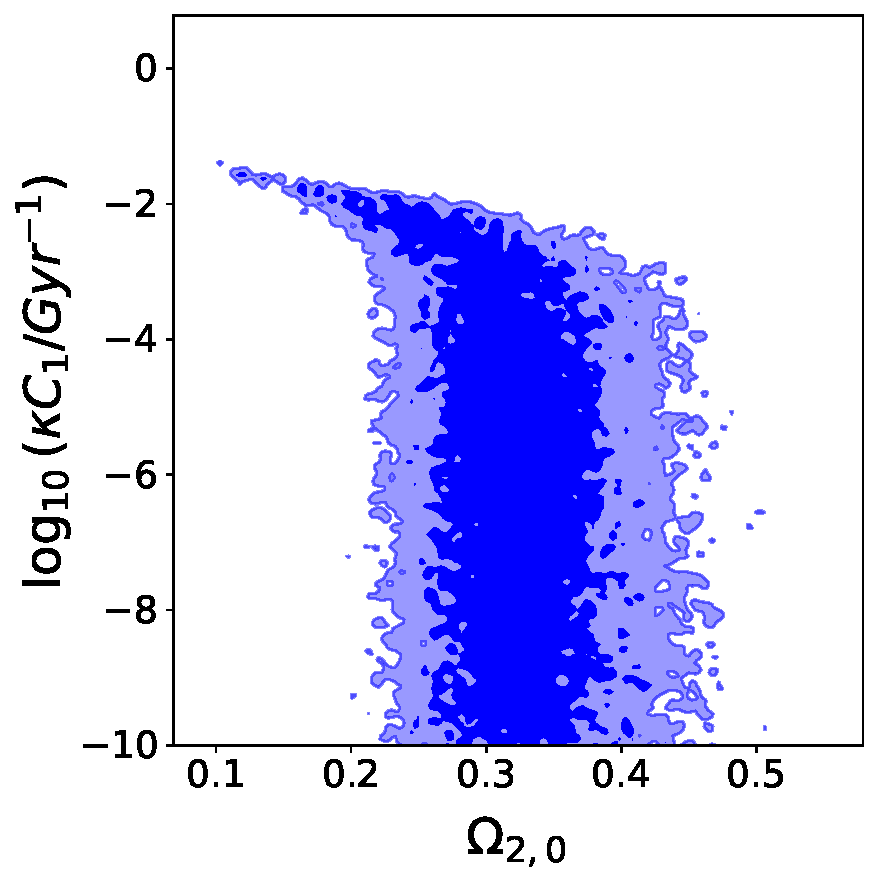
\includegraphics[width=0.22\textwidth]{ohd_1.pdf}
      }
      \subfigure{
         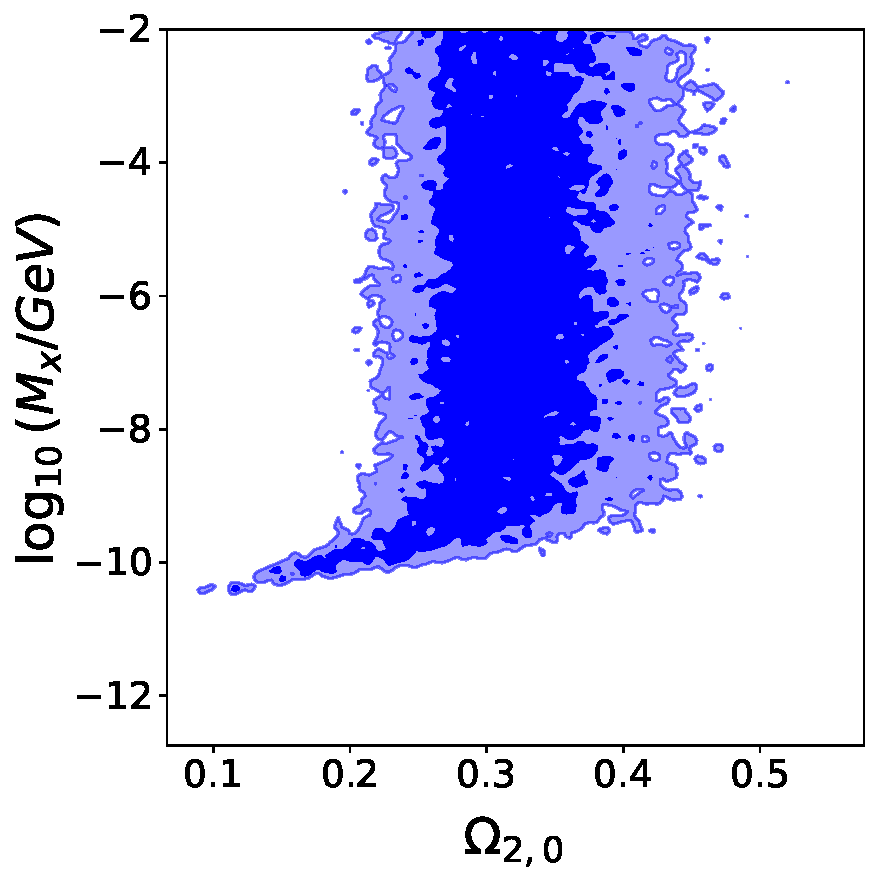
\includegraphics[width=0.22\textwidth]{ohd_2.pdf}
      }
      \caption{The constraint result from the observational
      $H(z)$ data.}
      \label{fig:1}
   \end{figure}

   \begin{figure}[htbp]
      \centering
      \subfigure{
         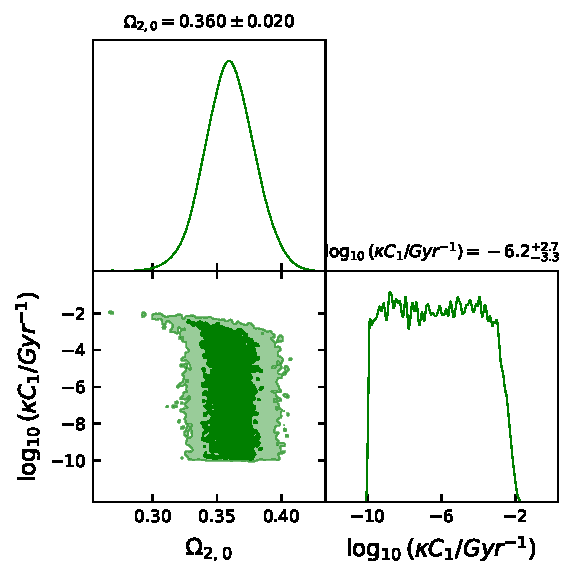
\includegraphics[width=0.22\textwidth]{sne_1.pdf}
      }
      \subfigure{
         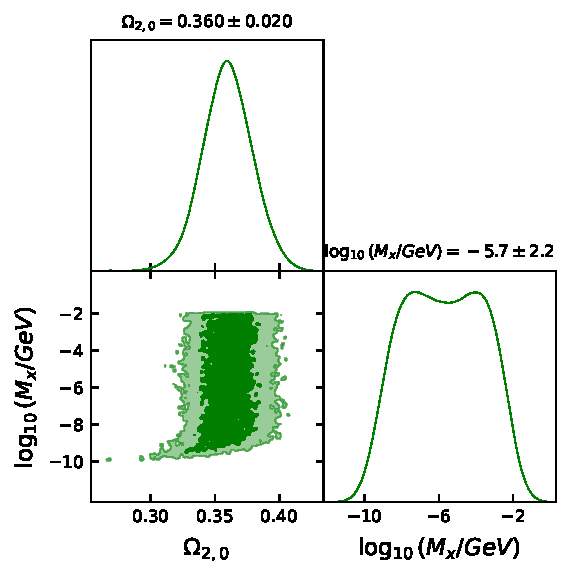
\includegraphics[width=0.22\textwidth]{sne_2.pdf}
      }
      \caption{The constraint result from the supernovae
      Ia data.}
   \end{figure}

   \begin{figure}[htbp]
      \centering
      \subfigure{
         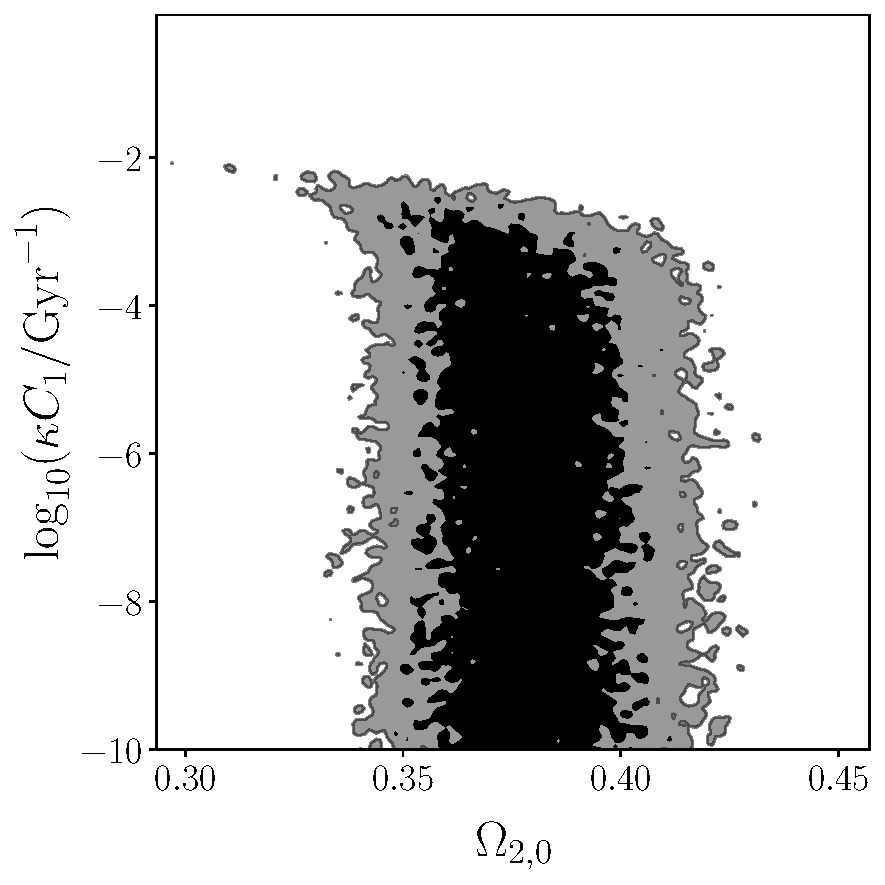
\includegraphics[width=0.22\textwidth]{sne_qso_1.pdf}
      }
      \subfigure{
         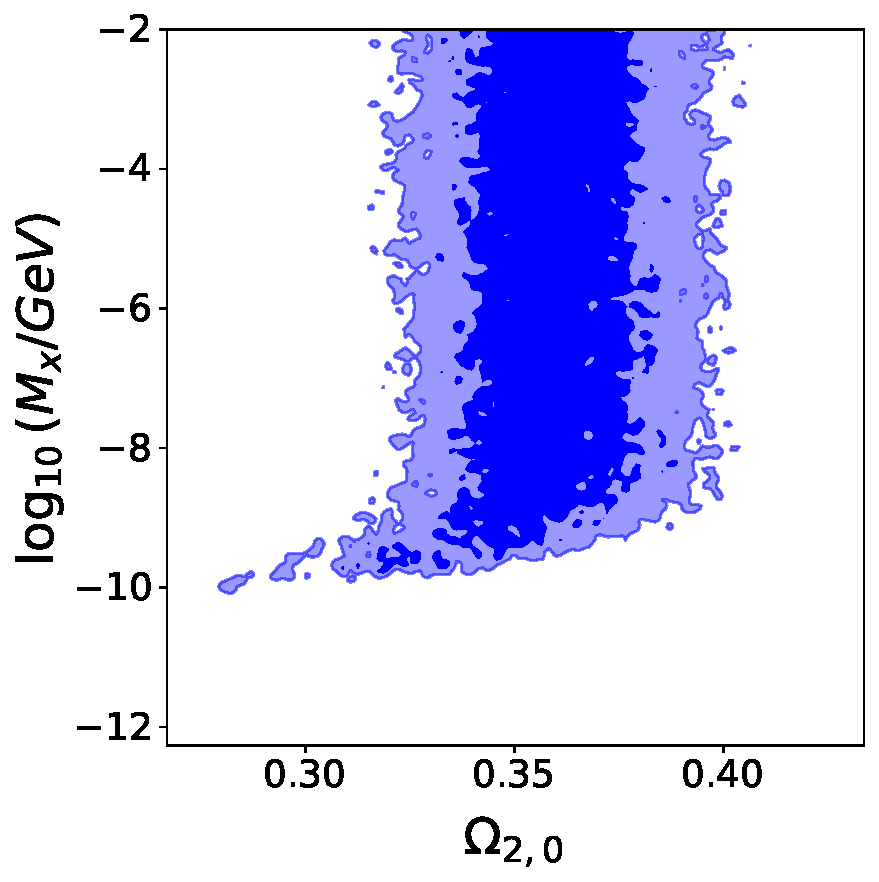
\includegraphics[width=0.22\textwidth]{sne_qso_2.pdf}
      }
      \caption{The constraint result from the SNe Ia + QSO data.}
   \end{figure}

   We could find that the combined result of SNe Ia and QSO is most
   similar to SNe Ia result, what may refer that the QSO cannot
   give an effective constraint. It may be due to the data quality
   at the high redshift, while the effective redshift of QSO as tracers in BAO
   is about 1.5, within the SNe Ia range.

   \begin{figure}[htbp]
      \centering
      \subfigure{
         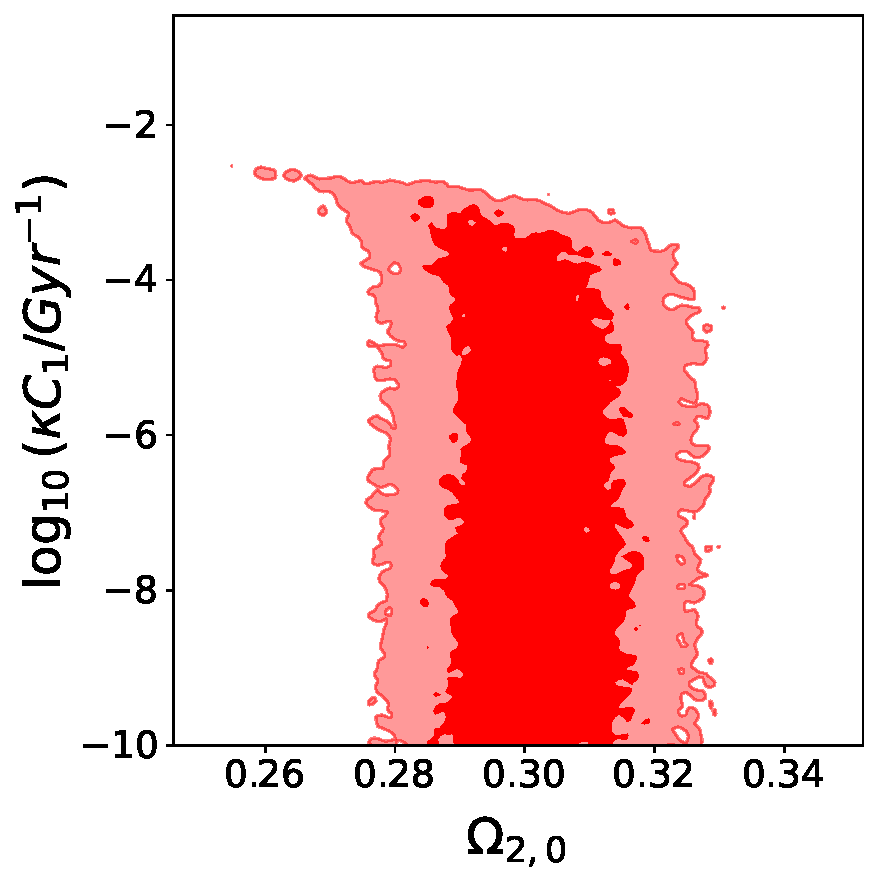
\includegraphics[width=0.22\textwidth]{bao_1.pdf}
      }
      \subfigure{
         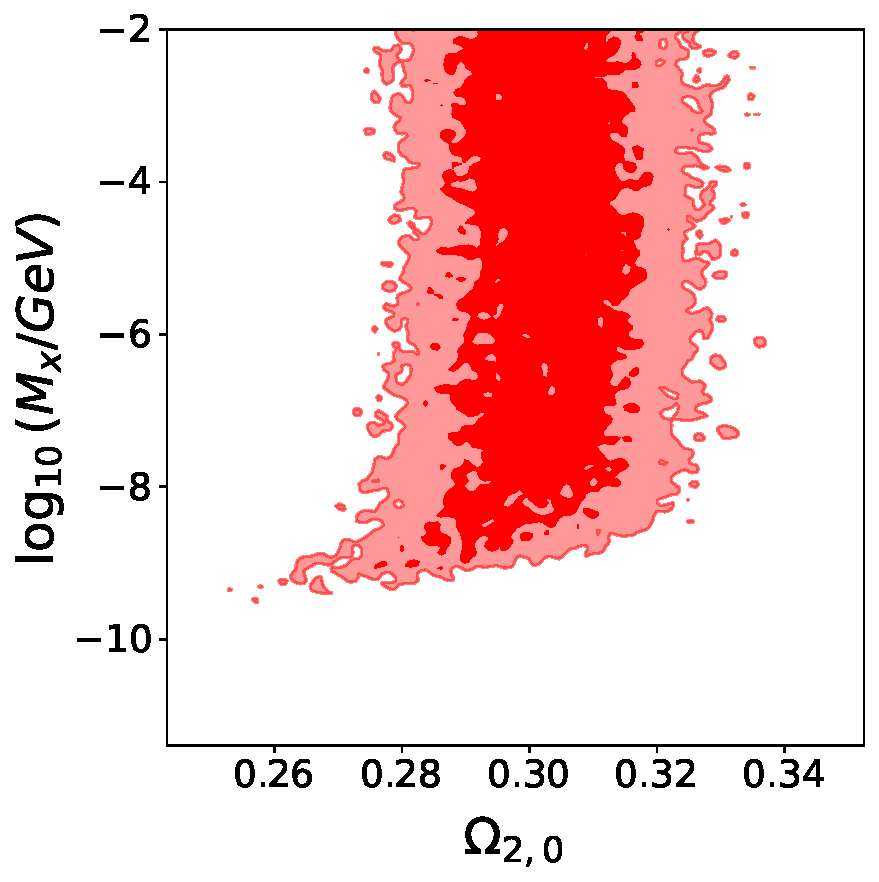
\includegraphics[width=0.22\textwidth]{bao_2.pdf}
      }
      \caption{The constraint result from the BAO data.}
   \end{figure}

   \begin{figure}[htbp]
      \centering
      \subfigure{
         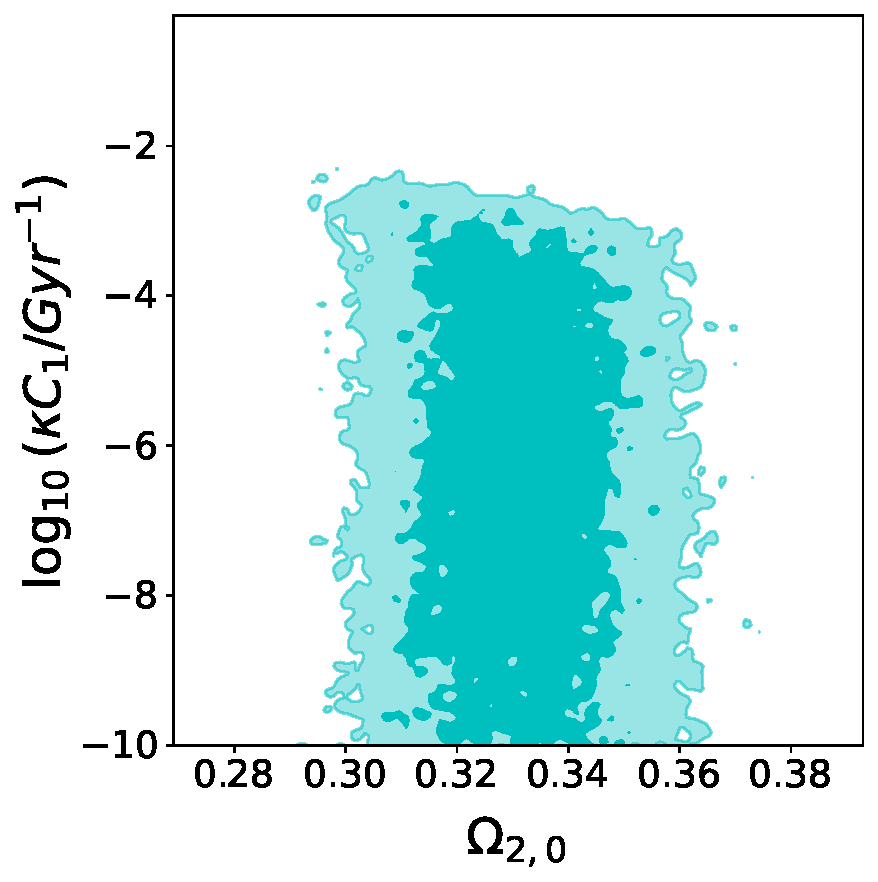
\includegraphics[width=0.22\textwidth]{ohd_sne_1.pdf}
      }
      \subfigure{
         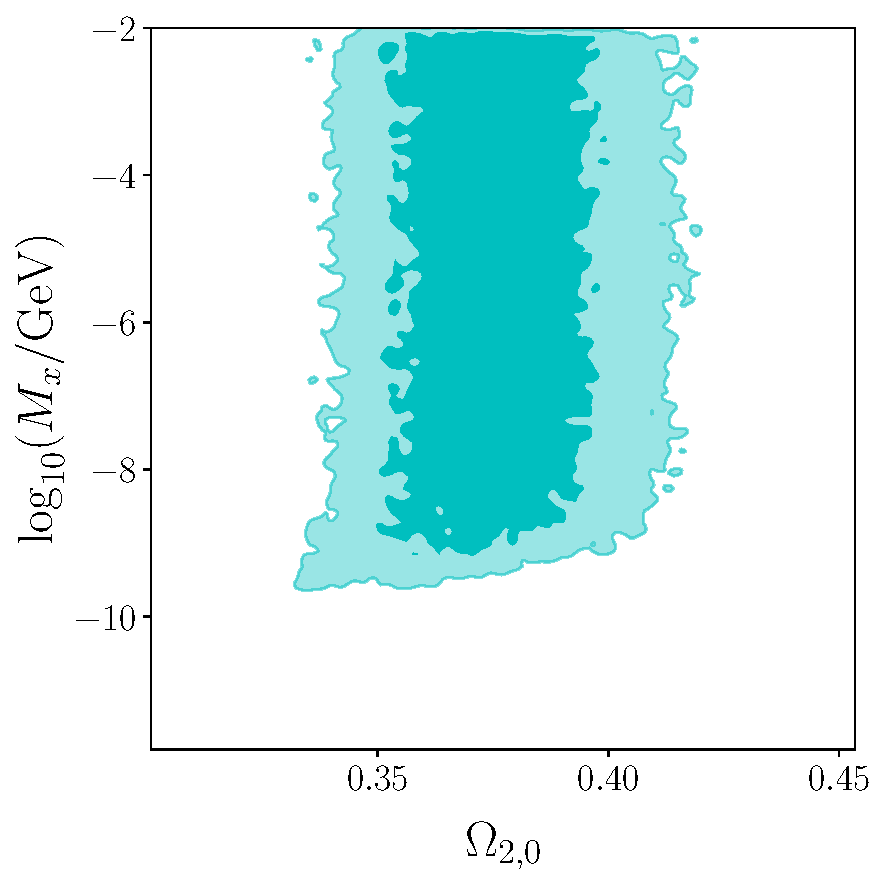
\includegraphics[width=0.22\textwidth]{ohd_sne_2.pdf}
      }
      \caption{The constraint result from the OHD + SNe Ia data.}
   \end{figure}

   \begin{figure}[htbp]
      \centering
      \subfigure{
         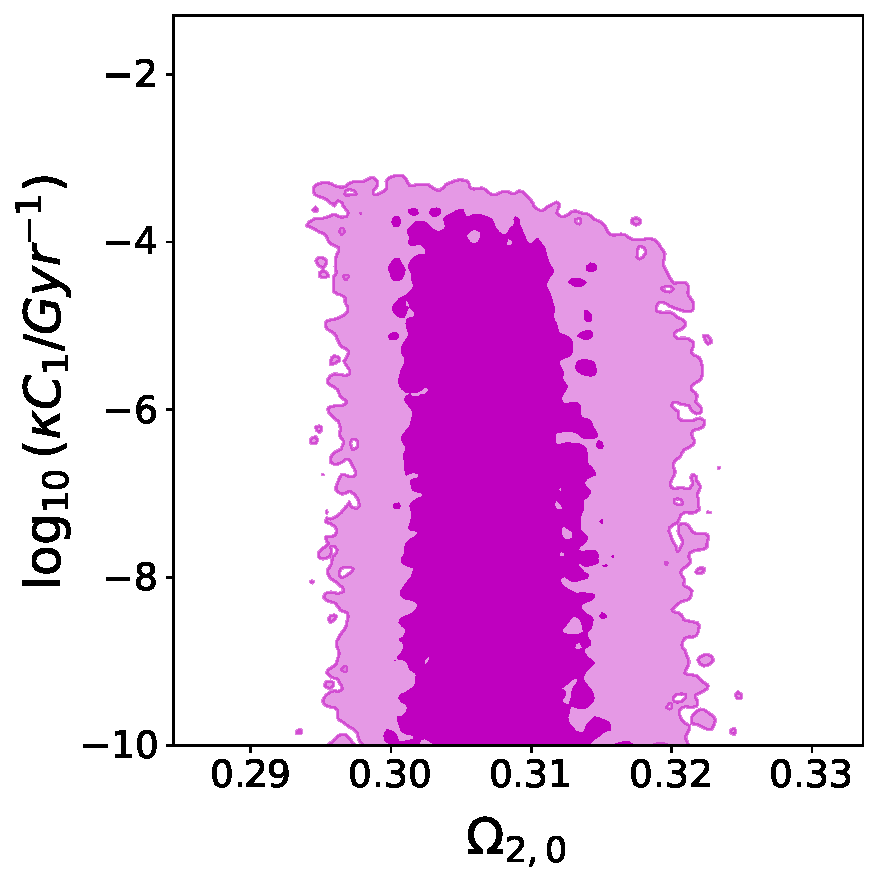
\includegraphics[width=0.22\textwidth]{ohd_sne_bao_1.pdf}
      }
      \subfigure{
         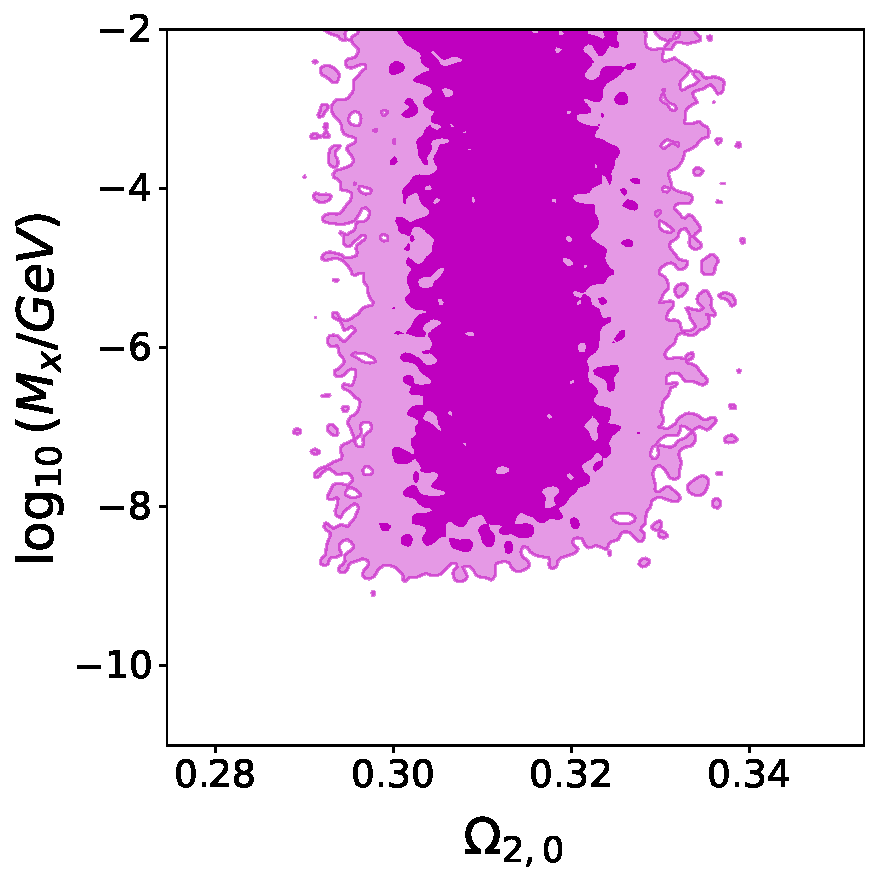
\includegraphics[width=0.22\textwidth]{ohd_sne_bao_2.pdf}
      }
      \caption{The constraint result from the OHD + SNe Ia + BAO data.}
      \label{fig:6}
   \end{figure}

   \begin{table*}[htbp]
      \centering
      \begin{tabular}{lcccccc}
         \hline\hline
         Model 1 & OHD & SNe Ia & SNe Ia + QSO & BAO &
          OHD + SNe Ia & OHD + SNe Ia + BAO \\
         \hline
         $\Omega_{2,0}$ & $0.321_{-0.067}^{+0.055}$ & $0.360_{-0.020}^{+0.020}$
          & $0.359_{-0.020}^{+0.020}$ & $0.301_{-0.013}^{+0.013}$
          & $0.330_{-0.016}^{+0.016}$ & $0.313_{-0.010}^{+0.010}$ \\
         $\log_{10}(\kappa C_1/$Gyr${}^{-1})$ & $<-2.17$ & $<-2.51$ & $<-2.57$
          & $<-3.10$ & $<-2.88$ & $<-3.39$ \\
         $\log_{10}(M_x/$GeV) & $>-9.77$ & $>-9.42$ & $>-9.40$
          & $>-8.84$ & $>-9.03$ & $>-8.52$ \\
         \hline
      \end{tabular}
      \caption{The constraint results of Model 1.}
      \label{tab:5}
   \end{table*}

\subsection{Model 2: mimicking the wCDM model}

   The constraint results of Model 2 are shown in Table \ref{tab:6}.

   \begin{figure}[htbp]
      \centering
      \subfigure{
         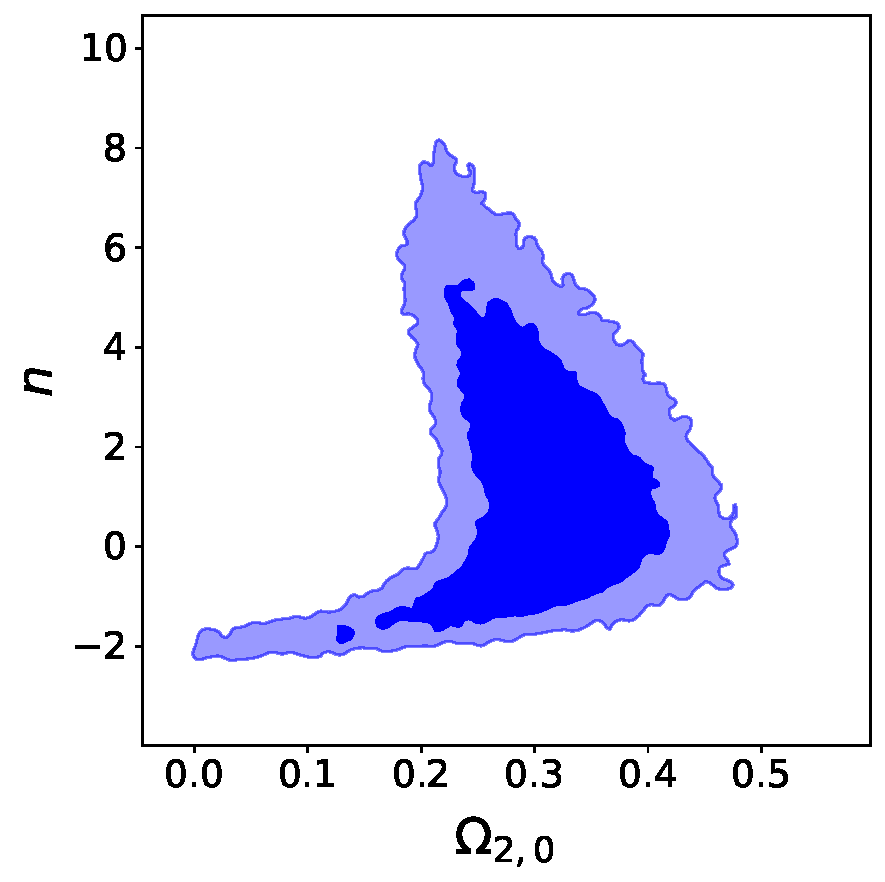
\includegraphics[width=0.22\textwidth]{ohd_widm_1.pdf}
      }
      \subfigure{
         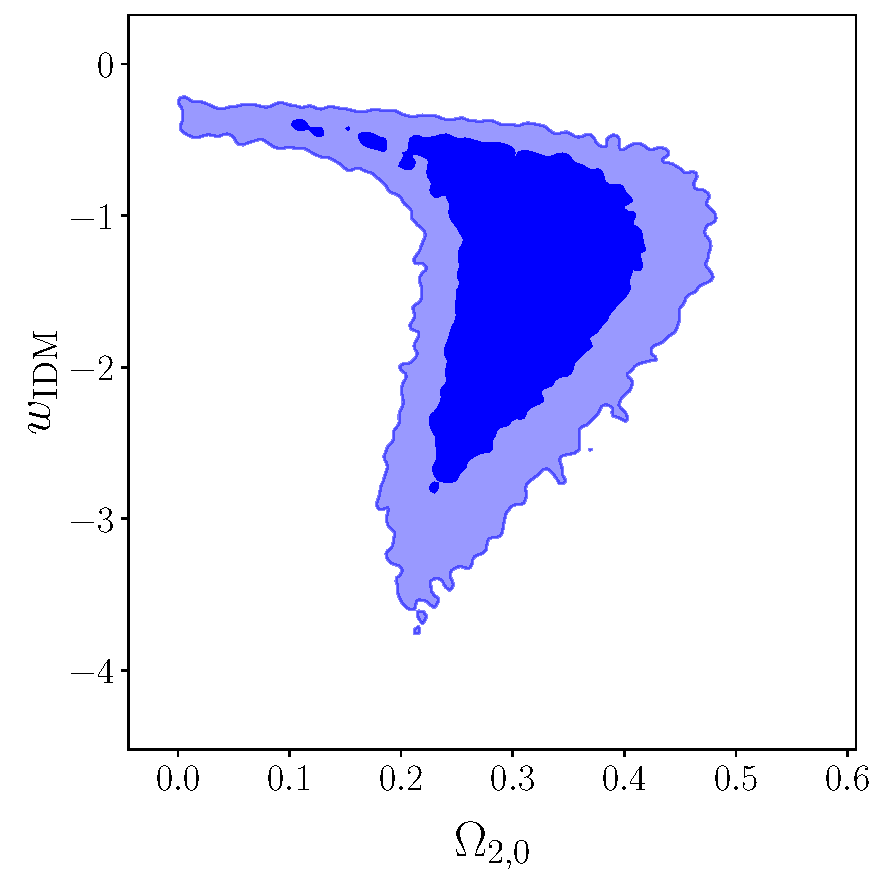
\includegraphics[width=0.22\textwidth]{ohd_widm_2.pdf}
      }
      \caption{The constraint result from the observational
      $H(z)$ data.}
   \end{figure}

   \begin{figure}[htbp]
      \centering
      \subfigure{
         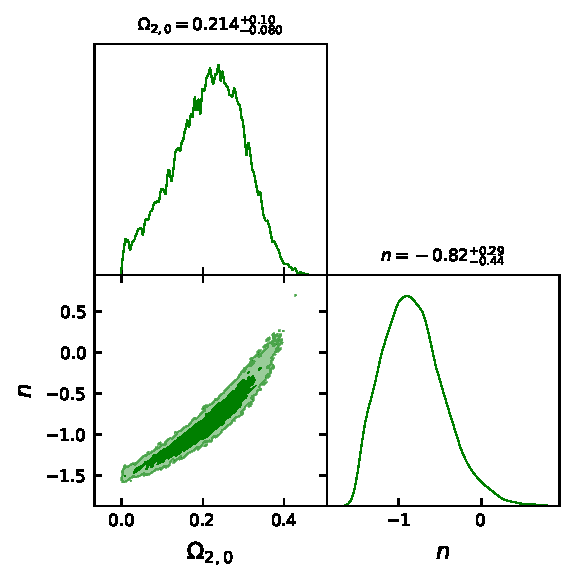
\includegraphics[width=0.22\textwidth]{sne_widm_1.pdf}
      }
      \subfigure{
         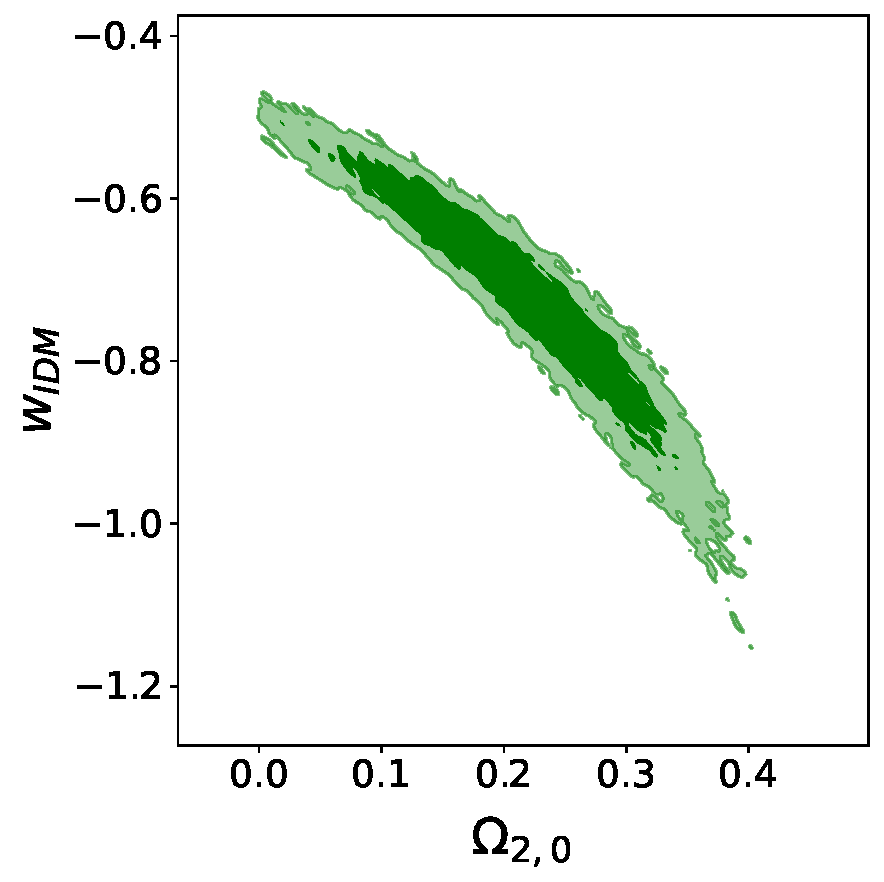
\includegraphics[width=0.22\textwidth]{sne_widm_2.pdf}
      }
      \caption{The constraint result from the supernovae
      Ia data.}
   \end{figure}

   \begin{figure}[htbp]
      \centering
      \subfigure{
         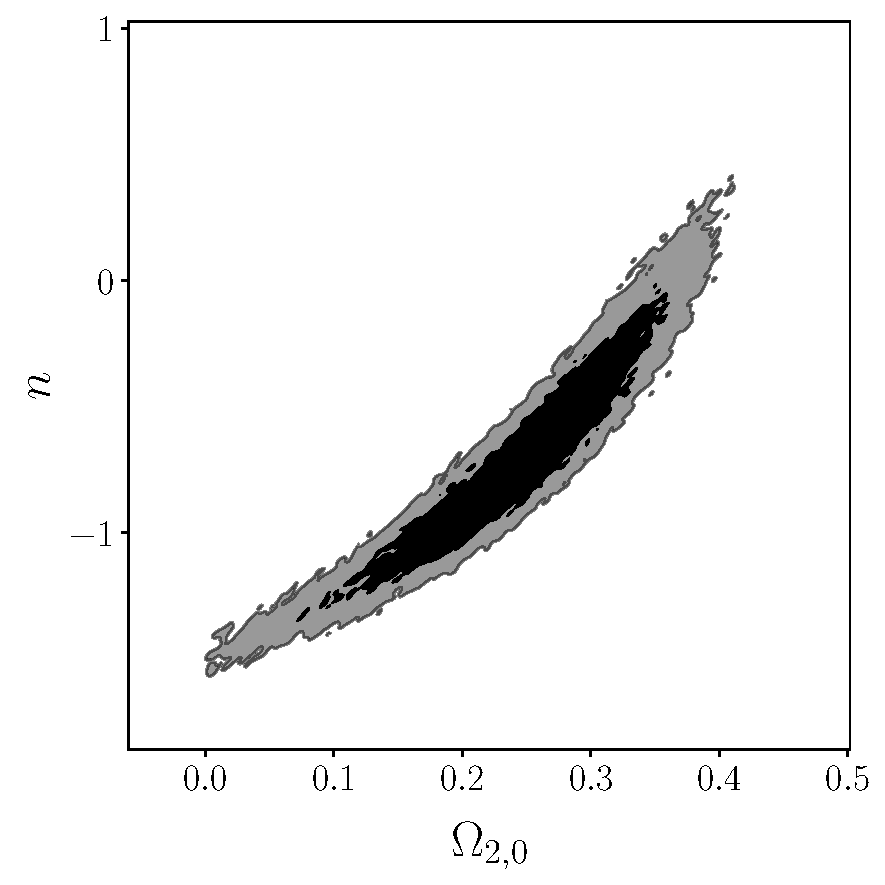
\includegraphics[width=0.22\textwidth]{sne_qso_widm_1.pdf}
      }
      \subfigure{
         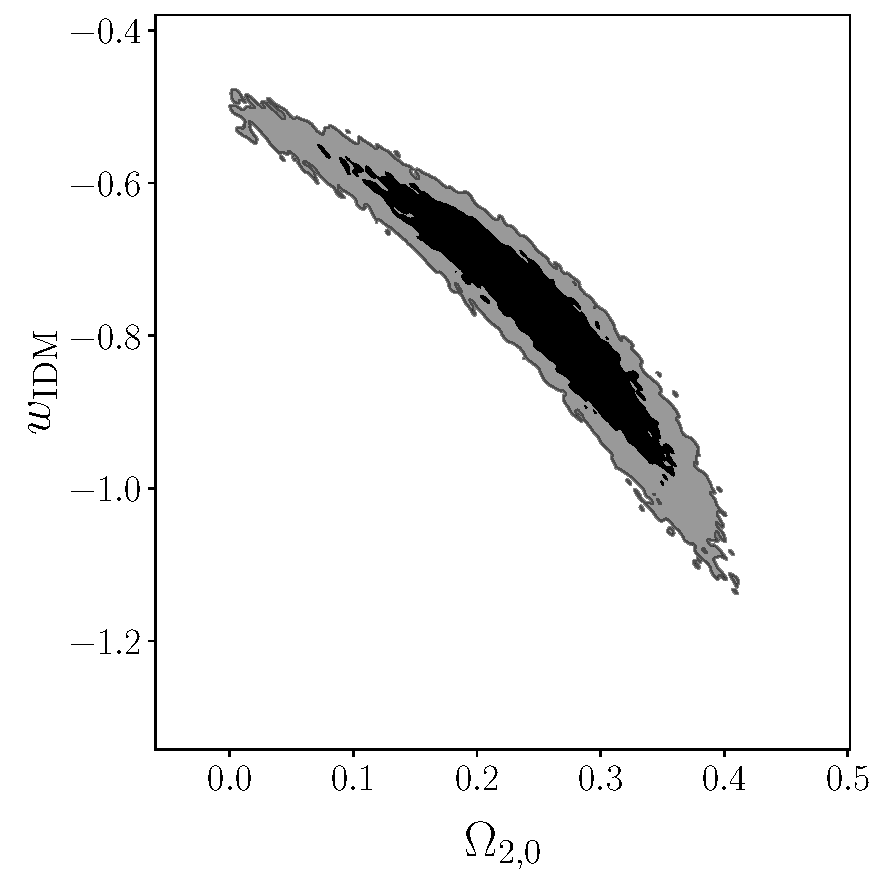
\includegraphics[width=0.22\textwidth]{sne_qso_widm_2.pdf}
      }
      \caption{The constraint result from the SNe Ia + QSO data.}
   \end{figure}

   \begin{figure}[htbp]
      \centering
      \subfigure{
         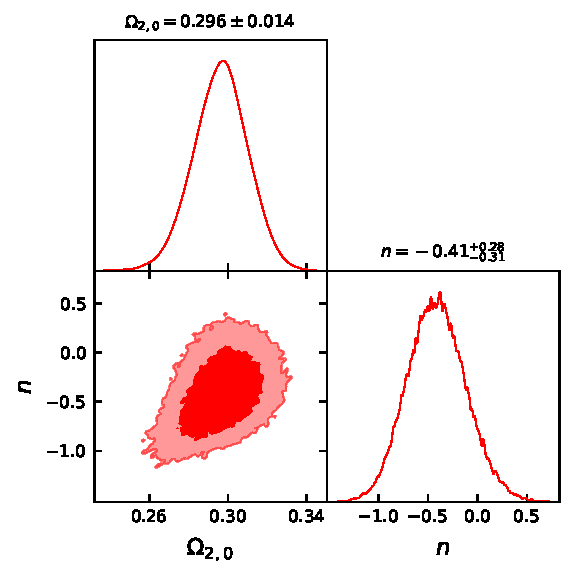
\includegraphics[width=0.22\textwidth]{bao_widm_1.pdf}
      }
      \subfigure{
         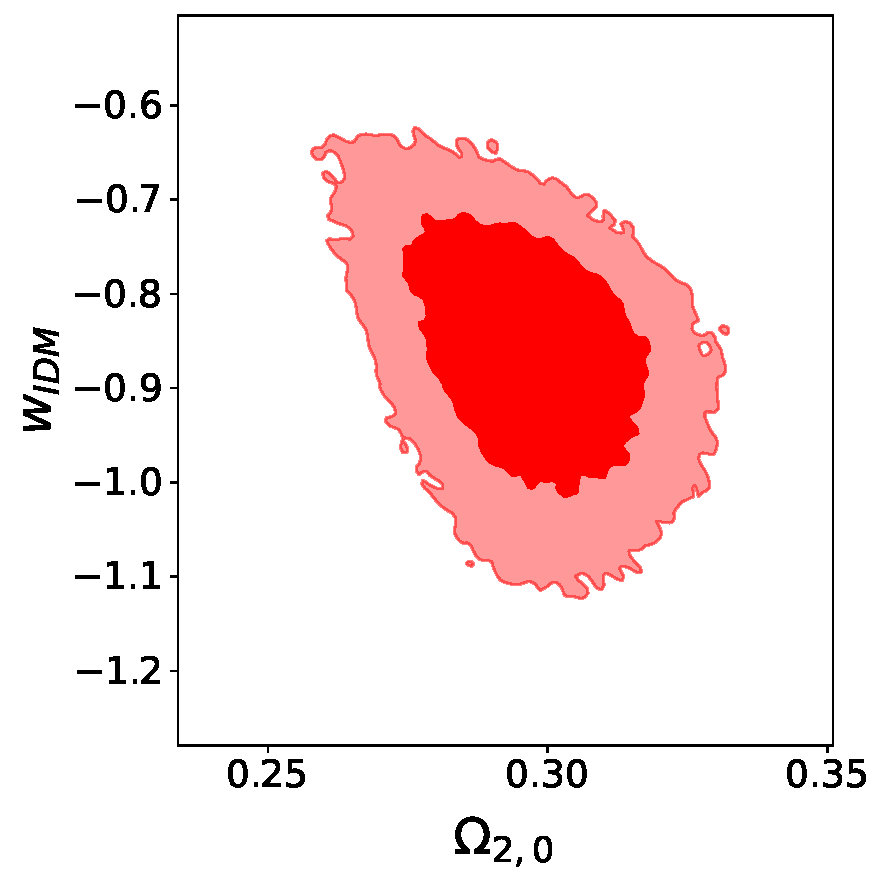
\includegraphics[width=0.22\textwidth]{bao_widm_2.pdf}
      }
      \caption{The constraint result from the BAO data.}
   \end{figure}

   \begin{figure}[htbp]
      \centering
      \subfigure{
         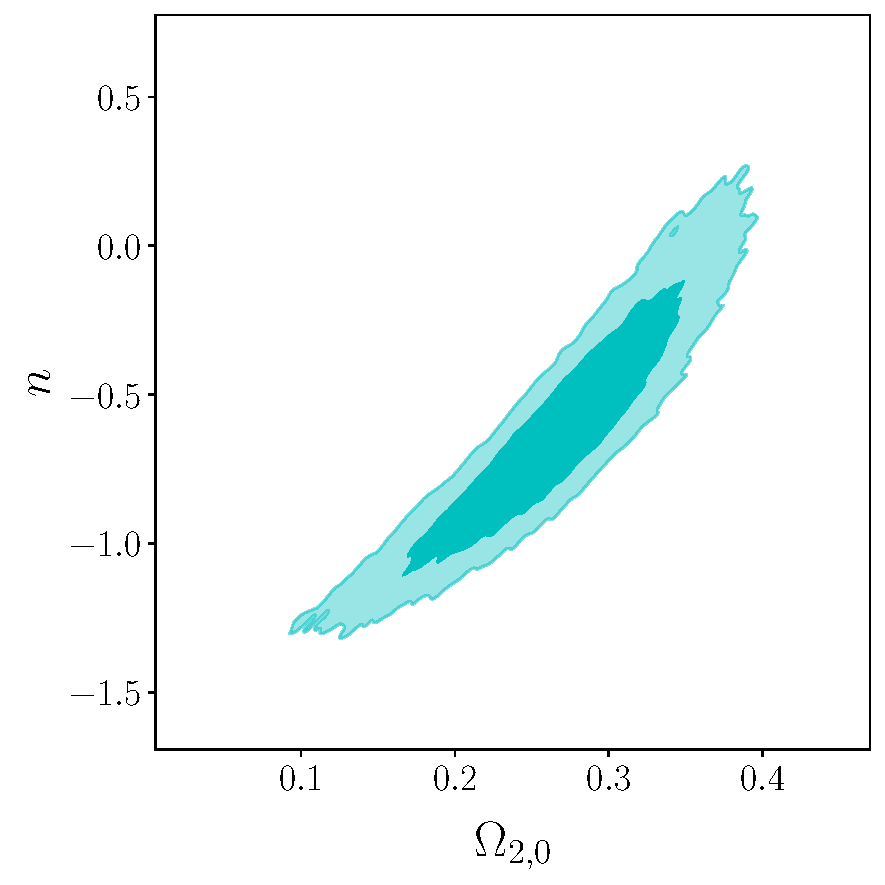
\includegraphics[width=0.22\textwidth]{ohd_sne_widm_1.pdf}
      }
      \subfigure{
         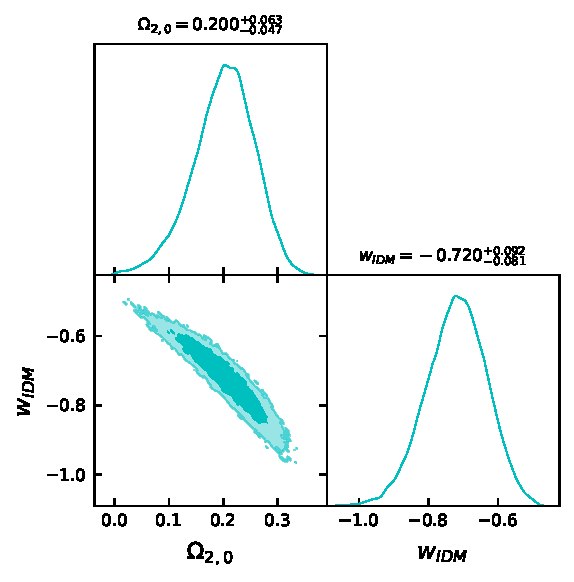
\includegraphics[width=0.22\textwidth]{ohd_sne_widm_2.pdf}
      }
      \caption{The constraint result from the OHD + SNe Ia data.}
   \end{figure}

   \begin{figure}[htbp]
      \centering
      \subfigure{
         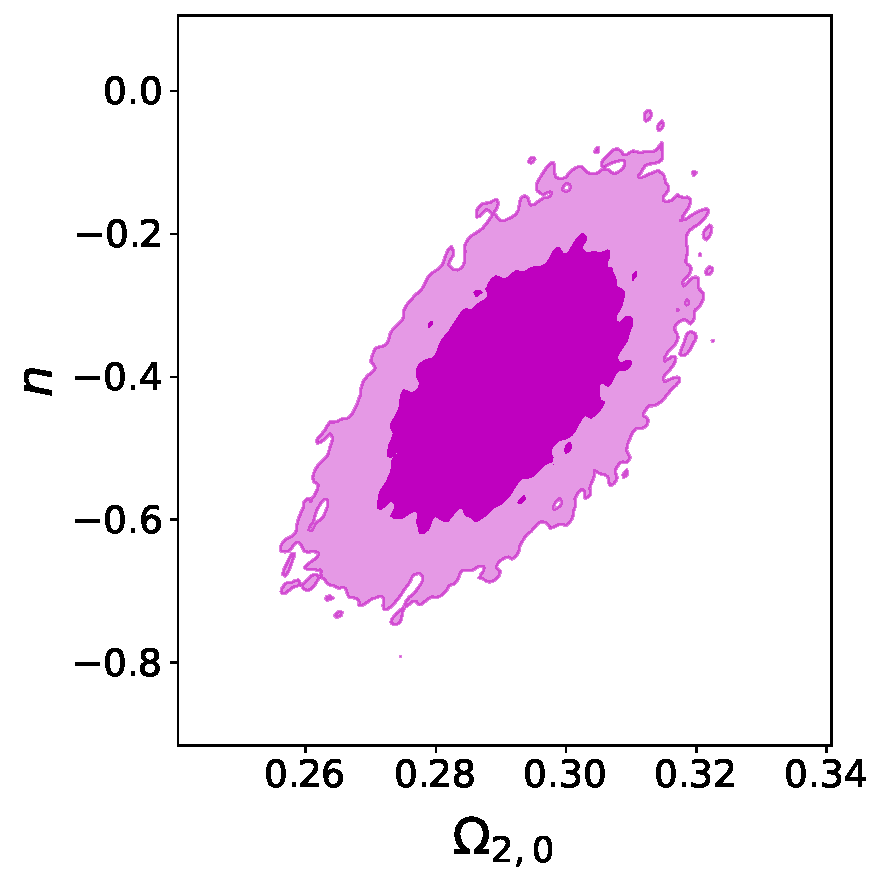
\includegraphics[width=0.22\textwidth]{ohd_sne_bao_widm_1.pdf}
      }
      \subfigure{
         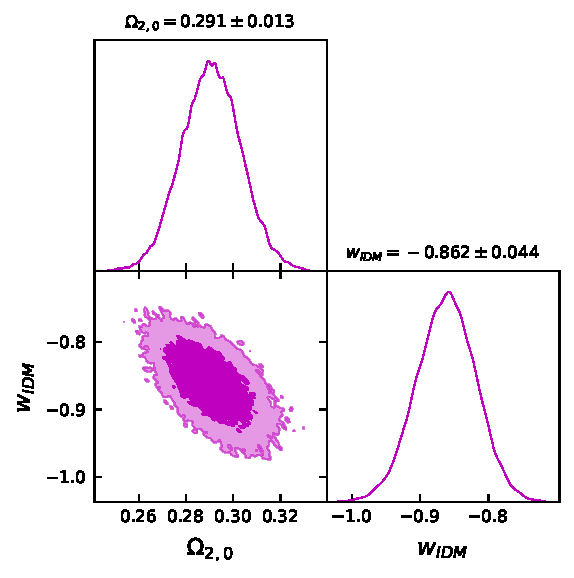
\includegraphics[width=0.22\textwidth]{ohd_sne_bao_widm_2.pdf}
      }
      \caption{The constraint result from the OHD + SNe Ia + BAO data.}
   \end{figure}

   The results from three dataset are different

   \begin{table*}[htbp]
      \centering
      \begin{tabular}{lcccccc}
         \hline\hline
         Model 2 & OHD & SNe Ia & SNe Ia + QSO & BAO &
          OHD + SNe Ia & OHD + SNe Ia + BAO \\
         \hline
         $\Omega_{2,0}$ & $0.295_{-0.077}^{+0.077}$ & $0.216_{-0.078}^{+0.096}$
          & $0.208_{-0.087}^{+0.12}$ & $0.296_{-0.014}^{+0.014}$
          & $0.202_{-0.049}^{+0.060}$ & $0.291_{-0.013}^{+0.013}$ \\
         $n$ & $1.4_{-2.8}^{+1.4}$ & $-0.82_{-0.44}^{+0.29}$
          & $-0.85_{-0.49}^{+0.42}$ & $-0.40_{-0.29}^{+0.29}$
          & $-0.83_{-0.27}^{+0.24}$ & $-0.41_{-0.13}^{+0.13}$ \\
         $w_{\text{IDM}}$ & $-1.5_{-0.9}^{+0.5}$ & $-0.73_{-0.15}^{+0.10}$
          & $-0.72_{-0.16}^{+0.14}$ & $-0.87_{-0.10}^{+0.10}$
          & $-0.72_{-0.09}^{+0.09}$ & $-0.86_{-0.04}^{+0.04}$ \\
         \hline
      \end{tabular}
      \caption{The constraint results of Model 2.}
      \label{tab:6}
   \end{table*}

\section{Conclusions}

\appendix

\section{The theoretical solution of model 1}

   Apply the Eq.(\ref{eq:12}) to Eq.(\ref{eq:8}), we can get a simple nonlinear
   second-order differential equation for the redshift $z(t)$, which can
   be written as \begin{equation}
      2H_0^2\Omega_{1,0}(1+z)^2z'z''+\kappa C_1z'{}^4-5H_0^2\Omega_{1,0}(1+z)z'{}^3
      +3H_0^4\Omega_{1,0}^2(1+z)^3z'-H_0^4\Omega_{1,0}^2\kappa C_1[(z+1)^4-1]
      =H_0^4\Omega_{1,0}^2\kappa C_1,
   \end{equation}
   where the prime denotes the derivative with respect to $t$.
   The equation can be simplified as
   \begin{equation}
      2H_0^2\Omega_{1,0}y^2y'y''+\kappa C_1y'{}^4-5H_0^2\Omega_{1,0}yy'{}^3
      +3H_0^4\Omega_{1,0}^2y^3y'-H_0^4\Omega_{1,0}^2\kappa C_1y^4=0,
   \end{equation}
   where $y=z+1$, now it is a homogeneous function and we can give the
   general solution as $y=\exp{f}$ with $f$ a function of $t$, the equation
   now is \begin{equation}
      2H_0^2\Omega_{1,0}f'f''+\kappa C_1f'{}^4-3H_0^2\Omega_{1,0}f'{}^3
      +3H_0^4\Omega_{1,0}^2f'-H_0^4\Omega_{1,0}^2\kappa C_1=0.
   \end{equation}
   We use $g=f'$, which also gives $g(t)=y'/y=-H(t)$, then the equation can be written as
   \begin{equation}
      2H_0^2\Omega_{1,0}gg'+\kappa C_1g^4-3H_0^2\Omega_{1,0}g^3
      +3H_0^4\Omega_{1,0}^2g-H_0^4\Omega_{1,0}^2\kappa C_1=0.
   \end{equation}
   It can be theoretically solved and the solution is like
   \begin{equation}
      g(t)=\mathcal{G}\left(-\frac{t}{2H_0^2\Omega_{1,0}}+Const\right),
   \end{equation}
   where $\mathcal{G}$ is the inverse function of
   \begin{equation}
      \mathcal{F}(x)=\frac{3H_0\sqrt{\Omega_{1,0}}\mathrm{arctanh}\frac{x}{H_0\sqrt{\Omega_{1,0}}}
      -\kappa C_1\log(x^2-H_0^2\Omega_{1,0})+\kappa C_1\log(\kappa C_1x^2-3H_0^2\Omega_{1,0}x
      +H_0^2\Omega_{1,0}\kappa C_1)}{9H_0^4\Omega_{1,0}^2-4H_0^2\Omega_{1,0}(\kappa C_1)^2}.
   \end{equation}
   In this term, $\displaystyle\mathrm{arctanh}(x)\doteq \frac{1}{2}\log\left(\frac{x+1}{x-1}\right)$
   when $x<-1$, and the $Const$ is determined by the boundary condition $g(0)\to -\infty$, which is

   \begin{equation}
      Const=\mathcal{F}(-\infty)\equiv\lim_{x\to-\infty}\mathcal{F}(x)=
      \frac{\kappa C_1\ln\kappa C_1}{9H_0^4\Omega_{1,0}^2-4H_0^2\Omega_{1,0}(\kappa C_1)^2}.
   \end{equation}
   The initial time of today $t_0$ can be easily given as
   \begin{equation}
      t_0=2H_0^2\Omega_{1,0}[\mathcal{F}(-\infty)-\mathcal{F}(-H_0)],
   \end{equation}
   and the redshift $z_{\max}$ can be calculated as
   \begin{equation}
      z_{\max}=\exp\left[2H_0^2\Omega_{1,0}\int_{-\infty}^{-H_0}[\mathcal{F}(-\infty)
      -\mathcal{F}(x)]\mathrm{d}x+H_0t_0\right]-1,
   \end{equation}
   and $z_{\max}$ is also a function of $\Omega_{2,0}, \kappa C_1$ and $H_0$.
   \begin{figure}[htbp]
      \centering
      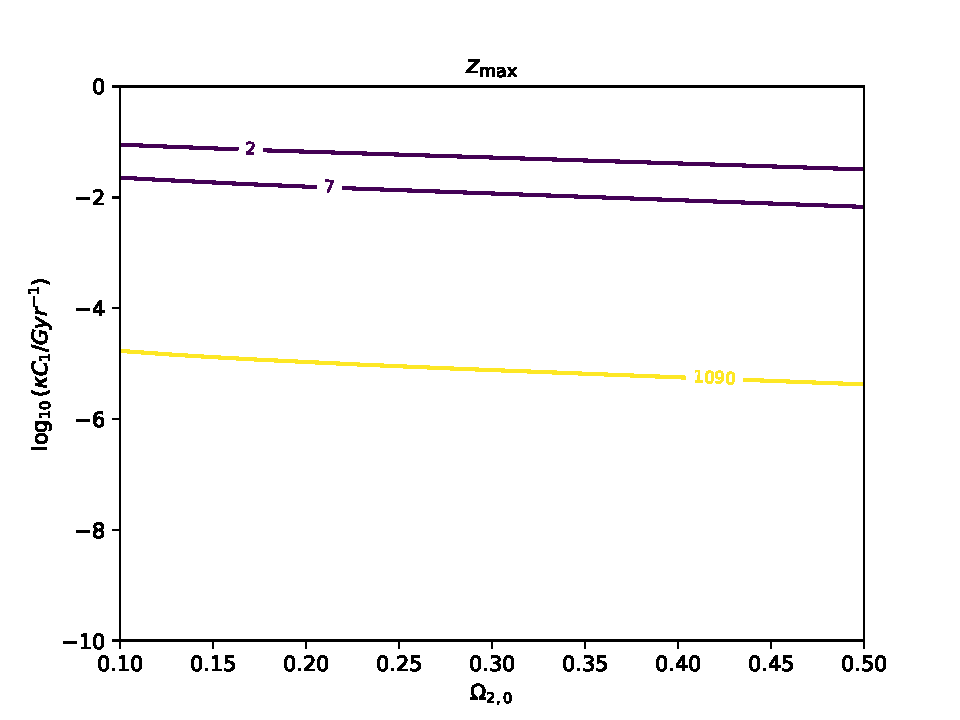
\includegraphics[width=0.7\textwidth]{zmax.pdf}
      \caption{The redshift $z_{\max}$ as $H_0=70$ km/s/Mpc}
   \end{figure}

\bibliography{reference}
\bibliographystyle{aasjournal}

\end{document}